\begin{figure}[H]
    \centering
    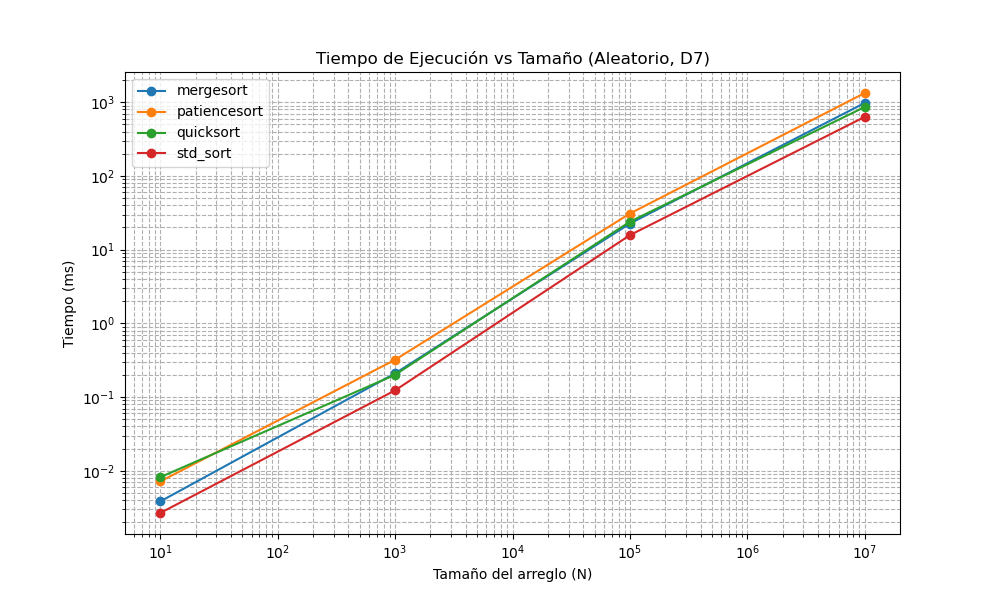
\includegraphics[width=1\textwidth]{../code/sorting/data/plots/sorting_aleatorio_D7.png}
    \caption{Tiempos de ejecucion empiricos para los algoritmos de ordenamiento (Caso Aleatorio, D7).}
    \label{fig:sorting}
\end{figure}

En la figura correspondiente al ordenamiento de arreglos aleatorios se observa que todos los algoritmos presentan una pendiente similar en la escala logaritmica confirmando graficamente su complejidad teorica de $O(n \log n)$. Sin embargo, sort domina consistentemente en todos los tamaños de arreglos ocupados. Esto se debe a la naturaleza hibrida que este posee, ademas de un buen uso de la memoria cache del procesador. QuickSort y MergeSort muestran un desempeño parejo, en arreglos de gran magnitud de datos practicamente se superponen entre si. Por otra parte, PatienceSort a pesar de tener un respaldo teorico positivo es el algoritmo que tiene mayor tiempo de ejecucion, probablemente debido a el gran costo computacional que genera la administracion constante de estructuras dinamicas y colas de prioridad.

\begin{figure}[H]
    \centering
    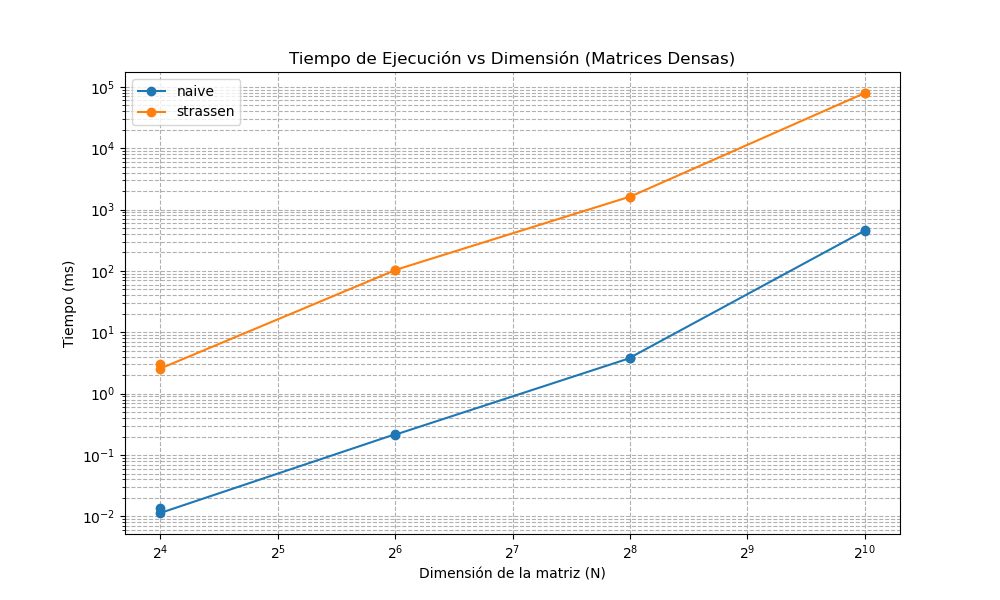
\includegraphics[width=1\textwidth]{../code/matrix_multiplication/data/plots/matrix_densa.png}
    \caption{Tiempos de ejecucion empiricos para la multiplicacion de matrices (Caso Denso).}
    \label{fig:matrix}
\end{figure}

En el analisis de las multiplicaciones de matrices densas, los resultados empiricos contrastan drasticamente con la expectativa teorica. En la teoria Strassen posee una cota asintotica superior al algoritmo Naive, sin embargo la grafica demuestra que la implementacion pura de strassen es constantemente mas lenta que el algoritmo Naive por varios ordenes de magnitud, alcanzando tiempos absurdamente lentos para las matrices de 1024. Esta baja de velocidad masiva se debe probablemente a las constantes ocultas de su recursion pura. Al dividir el problema hasta el caso base de $1 \times 1$, Strassen exige la instanciacion dinamica y copia millones de sub-vectores temporales en la RAM, esto provoca una saturacion en el sistema ralentizando el proceso considerablemente. Por el contrario, la implementacion Naive, optimizada en su bucle interno maximiza al iterar linealmente sobre la memoria.

\medskip

Al revisar los datos de memoria RAM en los resultados, notamos que para arreglos grandes, casi todos los algoritmos parecen consumir exactamente la misma cantidad de memoria (alrededor de 600 MB para arreglos de 10 millones). Sin embargo, esto ocurre por la forma en que el sistema mide los datos. La funcion de C++ que utilizamos no mide el consumo en cada milisegundo, sino que guarda el tope maximo de todo el programa. Como el codigo ejecuta los algoritmos uno detras de otro, los metodos que son muy eficientes con la memoria (sort o QuickSort) son "tapados" por la medicion mas grande registrada previamente. El principal responsable de esto es el PatienceSort y strassen en caso de las matrices, ya que constantemente piden al sistema crear miles de arreglos pequeños y estructuras dinamicas para poder funcionar. Aunque en la tabla de datos los numeros de RAM se ven repetidos por el mayor dato registrado, la prueba real de que la memoria colapso se ve en los graficos de tiempo, PatienceSort y strassen terminan siendo mucho mas lentos que sus contrapartes por todo el esfuerzo extra del sistema manejando la memoria pedida.